\documentclass[12pt,preprint]{aastex}
\usepackage{amssymb,amsmath}
%\usepackage{color,hyperref}
%\definecolor{linkcolor}{rgb}{0,0,0.25}
%\hypersetup{
%  colorlinks=true,        % false: boxed links; true: colored links
%  linkcolor=linkcolor,    % color of internal links
%  citecolor=linkcolor,    % color of links to bibliography
%  filecolor=linkcolor,    % color of file links
%  urlcolor=linkcolor      % color of external links
%}
\setlength{\emergencystretch}{2em}%No overflowing references
\newcommand{\ie}{i.e.}
\newcommand{\etal}{et al.}
\newcommand{\eg}{e.g.}
\newcommand{\eqnname}{equation}
\newcommand{\figurenames}{\figurename s}
\newcommand{\sectionname}{$\mathsection$}
\newcommand{\tvector}[1]{\boldsymbol{\vec{#1}}}
\newcommand{\vx}{\tvector{x}}
\newcommand{\vv}{\tvector{v}}
\newcommand{\Gaia}{\emph{Gaia}}

\begin{document}

\title{Tracing the Hercules stream around the Galaxy}
\author{Jo~Bovy}%\altaffilmark{1,2}}
\affil{Center for Cosmology and Particle Physics, Department of Physics, New York University, 4 Washington Place, New York, NY 10003, USA}
\email{jb2777@nyu.edu}
%\altaffiltext{1}{Center for Cosmology and Particle Physics, Department of Physics,
%  New York University, 4 Washington Place, New York, NY 10003, USA}
%\altaffiltext{2}{Correspondence should be addressed to jo.bovy@nyu.edu~.}

\begin{abstract}
%Various dynamical scenarios related to the Milky Way's bar or spiral
%structure have been proposed to explain the existence of moving
%groups---clumps of co-moving stars---in the Solar neighborhood. Since
%the observed pattern of moving groups is very sensitive to the
%properties of the non-axisymmetric feature that creates them, these
%moving groups can be a powerful tool in constraining the dynamical
%structure of the inner Milky Way. However, at present the various
%models are hard to confirm and distinguish with observations of the
%local Galactic neighborhood. We show that future programs that survey
%the Milky Way disk's kinematics on a more global scale can distinguish
%between these models. By integrating orbits of stars in various
%steady-state and transient bar and spiral structure potentials that
%produce the pattern of moving groups observed in the Solar
%neighborhood, we predict the velocity distribution as a function of
%location in the Galactic disk. We identify the locations that
%distinguish most clearly between the various scenarios. Future
%infrared radial velocity surveys can probe the velocity distribution
%at these locations. We predict the distribution of radial velocities
%that can be directly compared to observations to establish the origin
%of the moving groups and to constrain the structural and dynamical
%parameters of the non-axisymmetric Milky Way potential.
\end{abstract}

\keywords{
  Galaxy: bulge
  ---  
  Galaxy: disk
  ---
  Galaxy: evolution
  ---
  Galaxy: fundamental parameters
  ---
  Galaxy: kinematics and dynamics
  ---
  Galaxy: structure
}

\section{Introduction}


baryon acoustic feature, coincidence problem

\section{Methodology}

We follow Dehnen's approach \citep{dehnen00a}. Only planar.


\section{Two-dimensional velocity distributions}


\section{The line-of-sight velocity distribution}


\section{Discussion}

\subsection{\Gaia}

\subsection{Radial velocity surveys}

SDSS-III Project Description\footnote{Available at
  \url{http://sdss3.org/collaboration/description.pdf}~.}

\begin{thebibliography}{}

%\bibitem[{{Binney} \& {Tremaine}(2008)}]{binneytremaine}
%{Binney},~J. \& {Tremaine},~S., 2008, {Galactic Dynamics: Second Edition}
%  (Princeton University Press)

\bibitem[Bailer-Jones(2008)]{bailerjones08a}
  Bailer-Jones, ~C.~A.~L., 2008,
  in IAU Symp.~254, ed.~J.~Andersen, J.~Bland-Hawthorn, and B.~Nordstr\"{o}m, (Dordrecht: Kluwer), 475  

\bibitem[Bensby \etal(2007)]{Bensby07a}
  Bensby,~T., \etal, 2007,
  \apjl, 655, L89

\bibitem[Blaauw(1970)]{Blaauw70a}
  Blaauw,~A., 1970, in IAU Symp.~38, ed.~W.~Becker \& I.~Kontopoulos (Dordrecht: Reidel), 199

\bibitem[Blitz \& Spergel(1991)]{blitz91a}
  Blitz,~L.~\& Spergel,~D.~N., 1991, \apj, 379, 631

\bibitem[Binney, Gerhard, \& Spergel(1997)]{binney97a}
  Binney,~J.~J., Gerhard,~O., \& Spergel,~D.~N., 1997,
  \mnras, 288, 365

\bibitem[Bissantz \& Gerhard(2002)]{bissantz02a}
  Bissantz,~N.~\& Gerhard,~O., 2002,
  \mnras, 330, 591

\bibitem[Bovy, Hogg, \& Roweis(2009)]{Bovy09a} Bovy,~J., Hogg,~D.~W., \& Roweis,~S.~T., 2009,
  \apj, 700, 1794

\bibitem[Bovy \& Hogg(2010)]{Bovy10a} Bovy,~J.~\& Hogg,~D.~W., 2010,
  \apj, in press

\bibitem[Caloi \etal(1999)]{caloi99a}
  Caloi,~V.~, \etal, 1999,
  \aap, 351, 925

\bibitem[Cole \& Weinberg(2002)]{cole02a}
  Cole,~A.~A.~\& Weinberg,~M.~D., 2002,
  \apjl, 574, L43

\bibitem[{{Dehnen}(1998)}]{Dehnen98b}
Dehnen,~W., 1998, \aj, 115, 2384

\bibitem[Dehnen(1999a)]{dehnen99a}
  Dehnen,~W., 1999a, \aj, 118, 1190

\bibitem[Dehnen(1999b)]{dehnen99b}
  Dehnen,~W., 1999b, \aj, 118, 1201

\bibitem[Dehnen(1999c)]{dehnen99c}
  Dehnen,~W., 1999c, \apj, 524, L35

\bibitem[Dehnen(2000)]{dehnen00a}
  Dehnen,~W., 2000, \aj, 119, 800

\bibitem[Fux(2001)]{fux01a}
  Fux,~R., 2001,
  \aap, 373, 511

\bibitem[Gardner \& Flynn(2010)]{gardner10a}
  Gardner,~E.~\& Flynn,~C., 2010,
  \mnras, in press

\bibitem[H\"{a}fner \etal(2000)]{hafner00}
  H\"{a}fner,~R., \etal, 2000,
  \mnras, 314, 433

\bibitem[Minchev \& Famaey(2009)]{minchev09a}
  Minchev,~I.~\& Famaey,~B., 2009,
  \apj L, submitted

\bibitem[Raboud \etal(1998)]{raboud98a}
  Raboud,~D., \etal, 1998,
  \aap, 335, L61

\bibitem[Shen \etal(2010)]{Shen10a}
  Shen,~J., \etal, 2010, \apj L, submitted

\bibitem[Sellwood \& Binney(2002)]{sellwood02a}
  Sellwood,~J.~A.~\& Binney,~J.J., 2002,
  \mnras, 336, 785

\bibitem[Shu(1969)]{shu69a}
  Shu,~F.~H., 1969,
  \apj, 158, 505

\bibitem[Skuljan, Hearnshaw, \& Cottrell(1999)]{Skuljan99a}
  Skuljan,~J., Hearnshaw,~J.~B., \& Cottrell,~P.~L., 1999, \mnras, 308, 731

\end{thebibliography}


\clearpage
\begin{figure}
\includegraphics[width=0.5\textwidth]{veldist.eps}
\caption{observed}\label{fig:obs}
\end{figure}

\clearpage
\begin{figure}
\includegraphics[width=\textwidth]{rphi2d.ps}
\caption{2D}\label{fig:rphi2d}
\end{figure}

\clearpage
\begin{figure}
\includegraphics[width=\textwidth]{rphi1d.ps}\\
\includegraphics[width=\textwidth]{rphi1d2.ps}
\caption{1D}\label{fig:rphi1d}
\end{figure}

\clearpage
\begin{figure}
\includegraphics[width=0.5\textwidth]{detecta.ps}
\includegraphics[width=0.5\textwidth]{detectb.ps}
\caption{detect}\label{fig:detect}
\end{figure}

\clearpage
\begin{figure}
\includegraphics[width=0.5\textwidth]{distuncertain.ps}
\includegraphics[width=0.5\textwidth]{df.ps}\\
\includegraphics[width=0.5\textwidth]{slope.ps}
\includegraphics[width=0.5\textwidth]{barstrength.ps}
\caption{1dvar}\label{fig:1dvar}
\end{figure}



\end{document}
